\documentclass[12pt, a4paper, oneside]{ctexart}
\usepackage{amsmath, amsthm, amssymb, graphicx}
\usepackage[bookmarks=true, colorlinks, citecolor=blue, linkcolor=black]{hyperref}
\usepackage[margin = 25mm]{geometry}
\usepackage{setspace}
\usepackage{listings}
\usepackage{cite}
\usepackage{xcolor}
\usepackage{float}

\definecolor{codegreen}{rgb}{0,0.6,0}
\definecolor{codegray}{rgb}{0.5,0.5,0.5}
\definecolor{codepurple}{rgb}{0.58,0,0.82}
\definecolor{backcolour}{rgb}{0.95,0.95,0.92}

\lstdefinestyle{mystyle}{
    backgroundcolor=\color{backcolour},   
    commentstyle=\color{codegreen},
    keywordstyle=\color{magenta},
    numberstyle=\tiny\color{codegray},
    stringstyle=\color{codepurple},
    basicstyle=\ttfamily\footnotesize,
    breakatwhitespace=false,         
    breaklines=true,                 
    captionpos=b,                    
    keepspaces=true,                 
    numbers=left,                    
    numbersep=5pt,                  
    showspaces=false,                
    showstringspaces=false,
    showtabs=false,                  
    tabsize=2
}

\lstset{style=mystyle}


\title{Use the Newton-Raphson method to solve non-linear equations}
\date{\today}
\author{phys.2001 孙陶庵 202011010101 }
\begin{document}
\begin{spacing}{2.0}
\tableofcontents
\maketitle
\section{Newton-Raphson method}
\subsection{code}
\begin{lstlisting}[language=Matlab, caption=Newton-Raphson method]
    clear
    x0 = [0.1,0.1,-0.1];
    eps = 1e-5;
    maxiter = 10;
    F = @(x)([3*x(1) - cos(x(2)*x(3)) - 1/2;
        x(1)^2 - 81*(x(2) + 0.1)^2 + sin(x(3)) + 1.06;
        exp(-x(1)*x(2)) + 20*x(3) + (10*pi - 3)/3]);
    J = @(x)([3 -x(3)*sin(x(2)*x(3)) -x(2)*sin(x(2)*x(3)); 
        2*x(1) -162*(x(2) + 0.1) cos(x(3));
        -x(2)*exp(-x(1)*x(2)) -x(1)*exp(-x(1)*x(2)) 20]);
    x = double(x0);
    for i = 1:maxiter
        Jx = J(x);
        Fx = F(x);
        delta = - Jx \ Fx;
        x = x + delta;
        if norm(delta) < eps
            return;
        end
    end
    x


if i == maxiter
    error('This method can''t execute');
end

    \end{lstlisting}
\subsection{Principle explanation\cite{key2}\cite{key3}}
在开始编写代码之前,我们需要了解该方法的工作原理。 Newton-Raphson 方法是实数和实复数域上方程的近似解。 此方法使用函数 $f(x)$ 的泰勒级数的前件求根方程 $f(x)=0$。 \\
首先选择一个接近函数$f(x)$的零点的$x_0$并计算对应的$f(x_0)$
以及切线 $f'(x_0)$ 的斜率(其中 $f'$ 表示函数 $f$ 的导数)。
然后我们计算通过点 $(x_0, f(x_0))$ 和 $f'(x_0)$ 的线的交点
轴和 $x$ 轴的 $x$ 坐标,它是以下方程的解。
\begin{center}
    $0= (x-x_0)\cdot f'(x_0)+f(x_0)$
\end{center}

我们将新获得的点的 $x$ 坐标命名为 $x_1$。
通常,$x_1$ 比 $x_0$ 更接近方程 $f(x)=0$ 的解。
所以我们现在可以从 $x_1$ 开始下一次迭代。 迭代方程可以简化为:
\begin{center}
    $x_{n+1} = x_n - \frac{f(x_n)}{f'(x_n)}$
\end{center}

已经证明,牛顿迭代法的二次收敛必须满足以下条件:
$f'(x)\ne 0$; 对于所有 $x\in I$,其中 $I$ 是
区间$[\alpha - \gamma, \alpha + \gamma]$,$x_0$在区间$I$内,
即 $ r \geqslant \left| a-x_0 \right|$;
$f''(x)$ 对于所有 $x\in I$ 都是连续的;$x_0$ 足够接近根 $\alpha$。
然而,上面的方法只是一个函数求解器。 如果我们想获得非线性“方程”的算法,如下所示:
\begin{center}
    $    \begin{cases}
            3x_{1} - \cos{(x_{2}x_{3})} - \frac{1}{2} = 0 \\
            x_{1}^{2} - 81(x_{2} + 0.1)^{2} + \sin(x_{3}) + 1.06 = 0 \\
            e^{-x_{1}x_{2}} + 20x_{3} + \frac{10\pi - 3}{3} = 0
        \end{cases} $       
\end{center}

然后我们需要将定义从 $f'(x_n)$ 扩展到 $\nabla f(x)$。 方程式的形式将更改如下\cite{enwiki:1141352419}:
\begin{center}
    $\begin{bmatrix}
        \dfrac{\partial \mathbf{f}}{\partial x_1} & \cdots & \dfrac{\partial \mathbf{f}}{\partial x_n}
      \end{bmatrix}
      = \begin{bmatrix}
        \nabla^{\mathrm T} f_1 \\  
        \vdots \\
        \nabla^{\mathrm T} f_m   
      \end{bmatrix}
      = \begin{bmatrix}
          \dfrac{\partial f_1}{\partial x_1} & \cdots & \dfrac{\partial f_1}{\partial x_n}\\
          \vdots                             & \ddots & \vdots\\
          \dfrac{\partial f_m}{\partial x_1} & \cdots & \dfrac{\partial f_m}{\partial x_n}
      \end{bmatrix}$
\end{center}
这个矩阵称为雅可比矩阵。 我们将得到:
\begin{center}
    $x_{n+1} = x_n - J^{-1}(x_n)f'(x_n)$
\end{center}
\subsection{code-explanation}
我们可以看到上面的代码。 我们先用匿名函数定义2个函数,F是原函数。
下一个“函数”是雅可比矩阵:
\begin{center}
    $J(x) = \begin{pmatrix}
        3 & -x_{3}\sin{(x_{2}x_{3})} & -x_{2}\sin{(x_{2}x_{3})} \\
        2x_{1} & -162(x_{2} + 0.1)\cos(x_{3}) & -x_{1}\exp{(-x_{1}x_{2})} \\
        -x_{2}\exp{(-x_{1}x_{2})} & -x_{1}\exp{(-x_{1}x_{2})} & 20
        \end{pmatrix}
        $
\end{center}
现在,我们可以得到最终的结果:
\begin{center}
$    \begin{pmatrix}
        0.5000 & 0.5000 & 0.3000 \\
        0.0000 & 0.0000 & -0.2000 \\
        -0.5236 & -0.5236 & -0.7236
        \end{pmatrix}
$        
\end{center}


\section{Gauss-Seidel method}

\begin{lstlisting}[language=Matlab, caption=Newton-Raphson method]
x = [0.1,0.1,-0.1];
eps = 1e-5;
err = 10;

while(err>eps)
    y = g(x);
    err = norm(y-x);
    x = y;
end

x

function y = g(x)
    y(1) = 1/3*cos(x(2)*x(3))+1/6;
    y(2) = 1/9*sqrt(x(1)^2+sin(x(3))+1.06)-0.1;
    y(3) = -exp(-x(1)*x(2))/20-(10*pi-3)/60;
end

\end{lstlisting}

上面的代码是从课程上来的。

\section{Jacobian method}
我真的很抱歉,但我真的不知道Gauss-Seidel算法和Jacobi算法之间的区别。
\section{Convergence speed for iterative methods}
收敛速度的原理在reference\cite{key1}中已经提及,这里不再赘述。
\subsection{Newton-Raphson method}
\begin{lstlisting}[language=Matlab, caption=Newton-Raphson method with Convergence speed for iterative methods] 
    clear
    x0 = [0.1,0.1,-0.1];
    eps = 1e-5;
    maxiter = 10;
    F = @(x)([3*x(1) - cos(x(2)*x(3)) - 1/2;
        x(1)^2 - 81*(x(2) + 0.1)^2 + sin(x(3)) + 1.06;
        exp(-x(1)*x(2)) + 20*x(3) + (10*pi - 3)/3]);
    J = @(x)([3 -x(3)*sin(x(2)*x(3)) -x(2)*sin(x(2)*x(3)); 
        2*x(1) -162*(x(2) + 0.1) cos(x(3));
        -x(2)*exp(-x(1)*x(2)) -x(1)*exp(-x(1)*x(2)) 20]);
    x = double(x0);
    alpha111 = zeros(1, maxiter);
    
    for i = 1:maxiter
        Jx = J(x);
        Fx = F(x);
        delta = - Jx \ Fx;
        x = x + delta;
        alpha111(i) = norm(Fx);
        if norm(delta) < eps
            break;
        end
    end
    semilogy(1:i, alpha111(1:i), 'o-');
    xlabel('Iteration');
    ylabel('alpha');    
\end{lstlisting}
\subsection{Gauss-Seidel method}
\begin{lstlisting}[caption=Gauss-Seidel method with Convergence speed for iterative methods] 
    x = [0.1,0.1,-0.1];
    eps = 1e-5;
    err = 10;
    order11 = [];
    
    while(err>eps)
        y = g(x);
        err = norm(y-x);
        order11 = [order11 err];
        x = y;
    end
    
    p = polyfit(log(order11(1:end-1)), log(order11(2:end)), 1);
    convergence_rate = p(1);
    
    semilogy(order11);
    title(['Convergence rate: ', num2str(convergence_rate)]);
    xlabel('Iteration');
    ylabel('Error');
    
    
    function y = g(x)
        y(1) = 1/3*cos(x(2)*x(3))+1/6;
        y(2) = 1/9*sqrt(x(1)^2+sin(x(3))+1.06)-0.1;
        y(3) = -exp(-x(1)*x(2))/20-(10*pi-3)/60;
    end
    

\end{lstlisting}
\subsection{Jacobi method}
\section{Convergence Rate Comparison of Different Algorithms}
\begin{figure}[H]
	\centering
	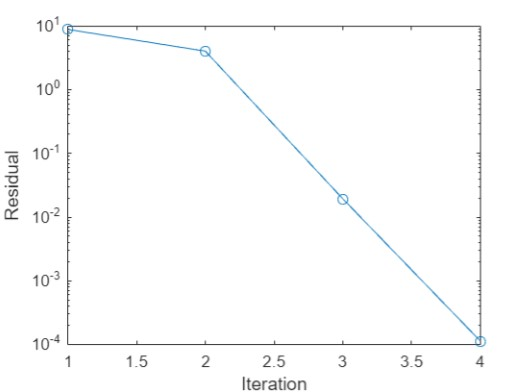
\includegraphics[width=8cm]{newtonlaw.jpg}
	\caption{newtonlaw}
\end{figure}
\begin{figure}[H]
	\centering
	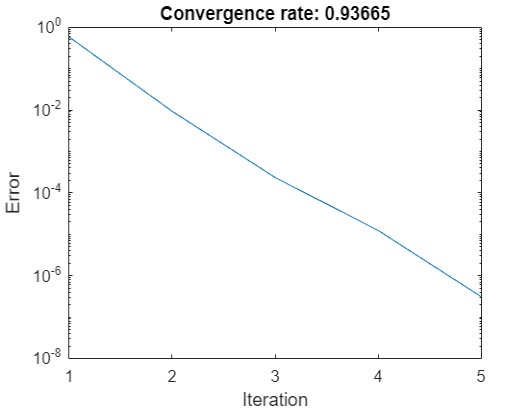
\includegraphics[width=8cm]{Gauss.jpg}
	\caption{Gauss}
\end{figure}

\end{spacing}{}

\bibliographystyle{IEEEtran}
\bibliography{alpha1}

\end{document}